\documentclass{standalone}
\usepackage[x11names, rgb, svgnames]{xcolor}
\usepackage[utf8]{inputenc}
\usepackage{tikz}
\usetikzlibrary{fit,snakes,arrows,shapes}
\usepackage{amsmath}
%
%

%

%

\begin{document}
\pagestyle{empty}
%
%
%

\enlargethispage{100cm}
% Start of code
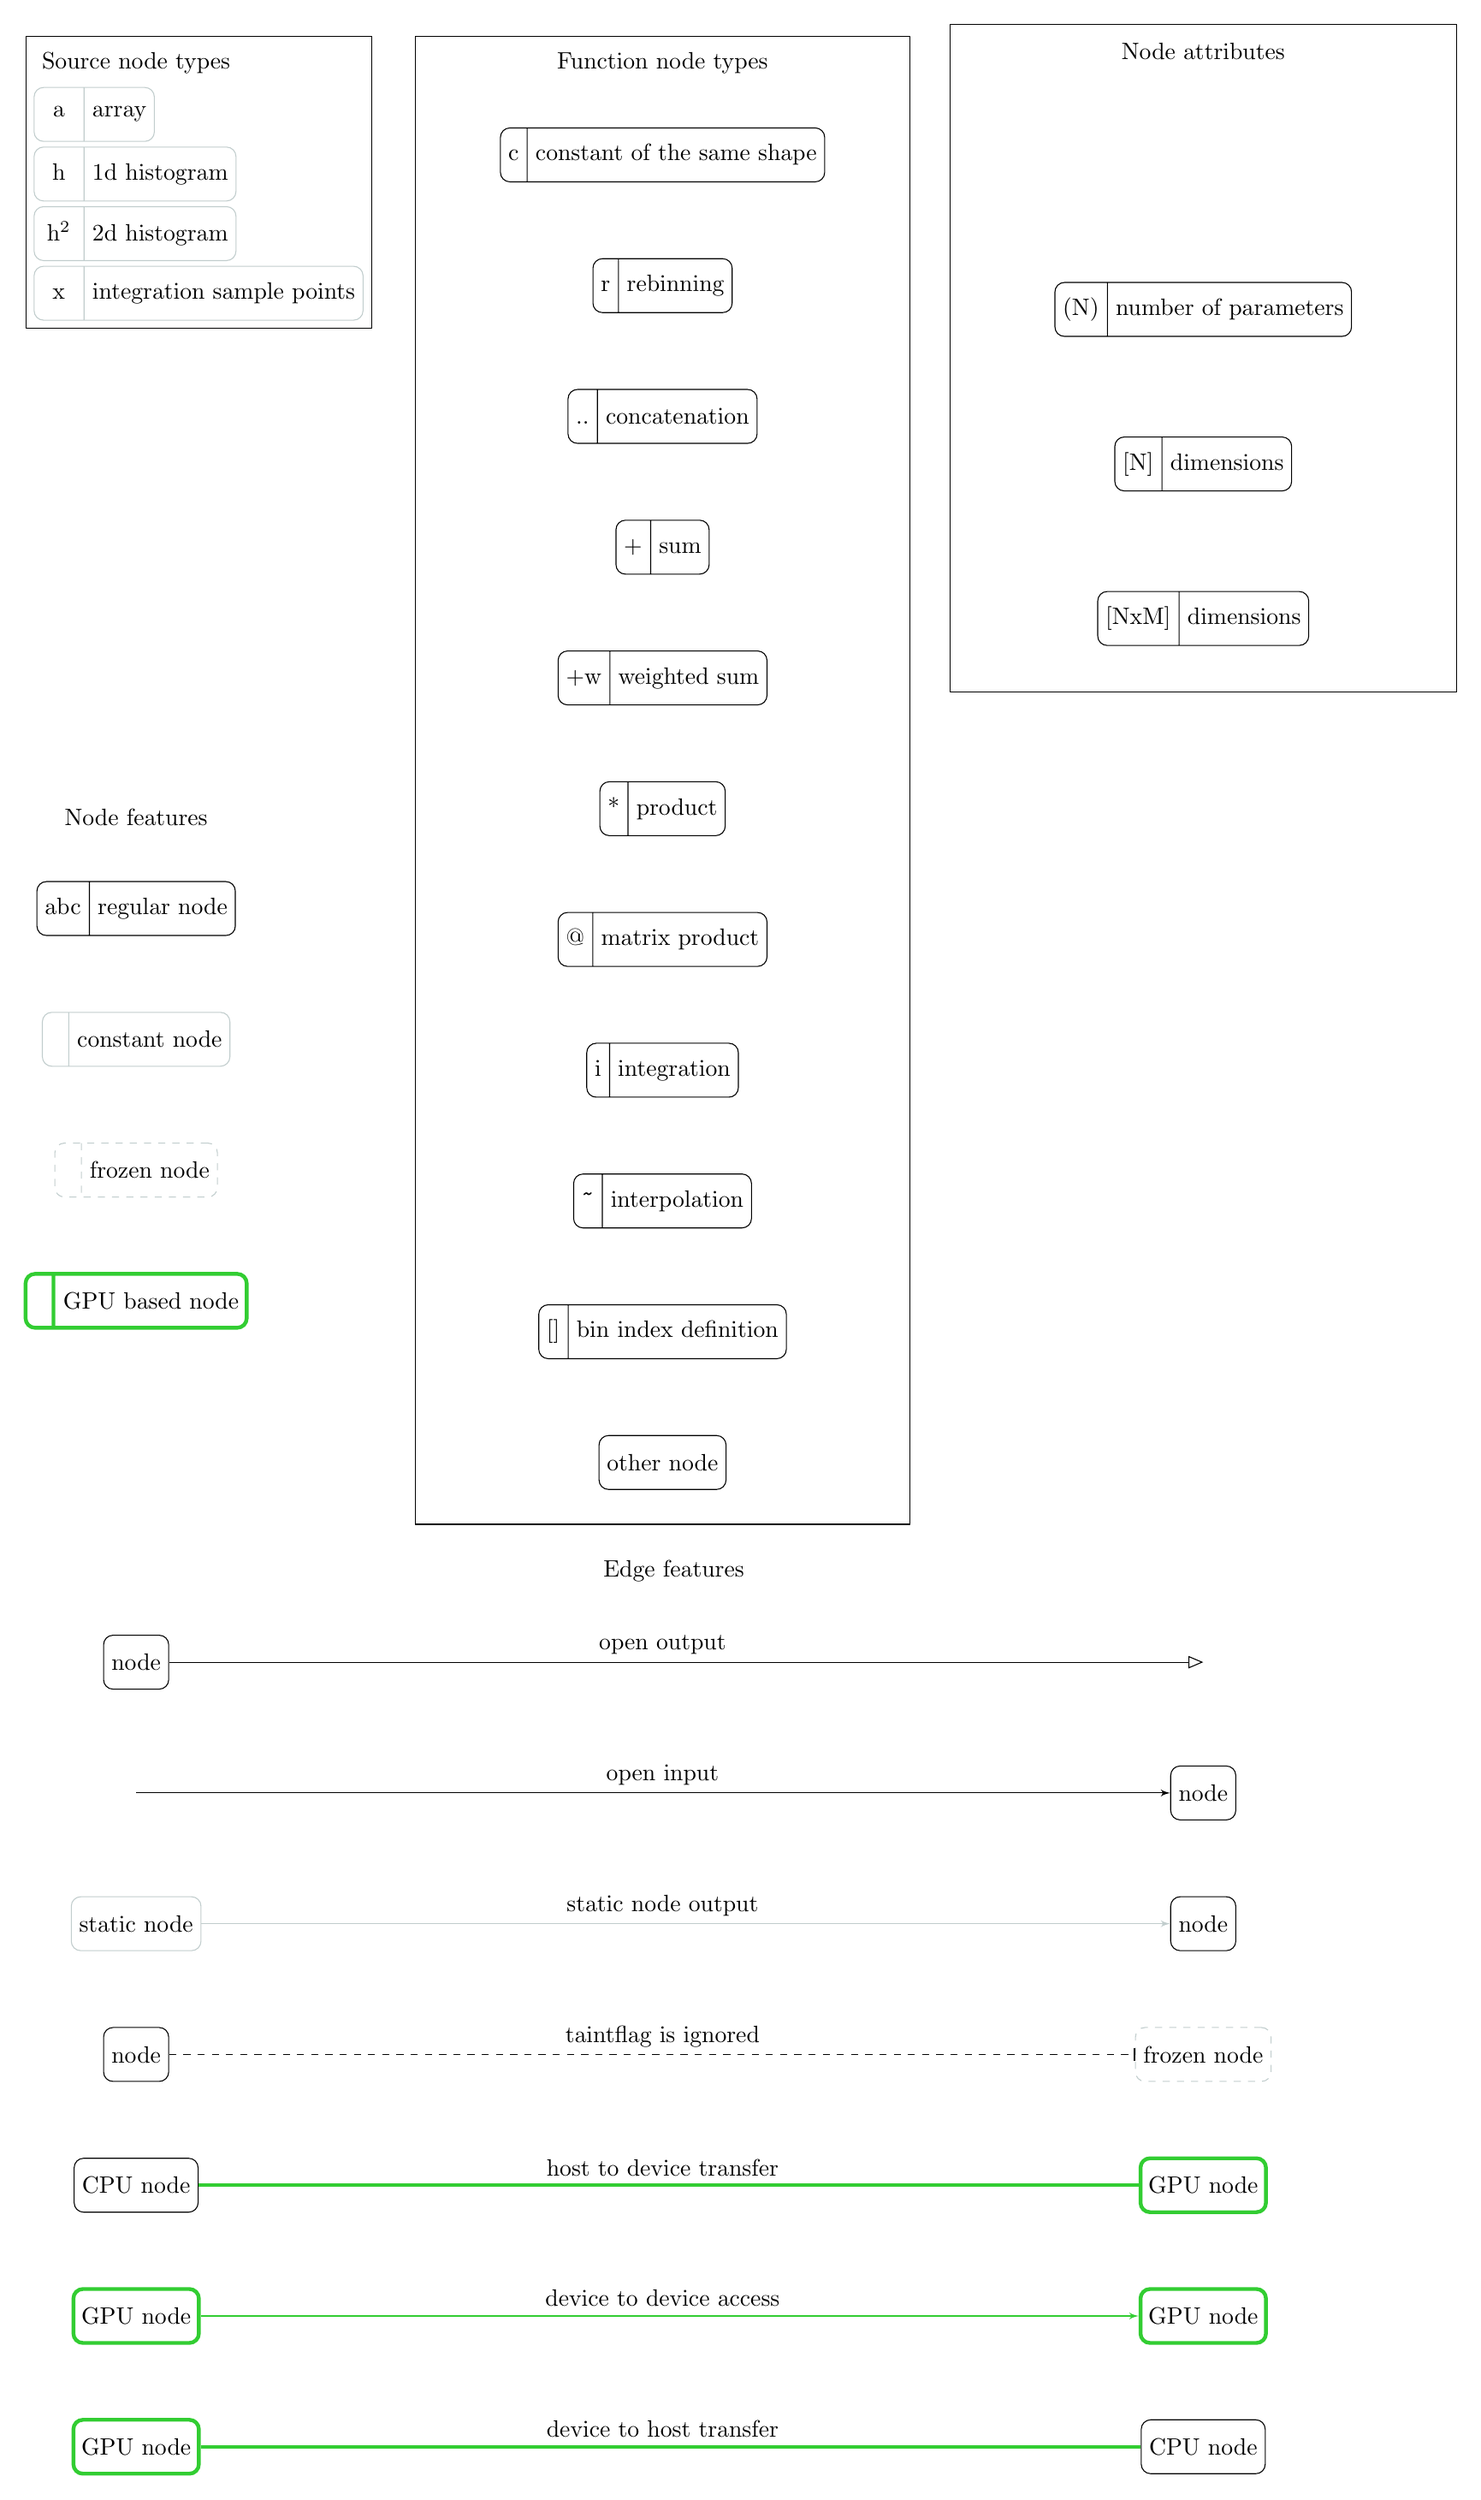
\begin{tikzpicture}[>=latex',line join=bevel,
  nodeshape/.style={rectangle split,
                    rectangle split horizontal,
                    rectangle split parts=#1,
                    rectangle split part align=base,
                    rounded corners,
                    minimum height=8mm},
  tapered/.style={ultra thick},
  gpu/.style={ultra thick,draw=LimeGreen},
  static/.style={draw=Azure3},
  ]
%%
\begin{scope}
  \pgfsetstrokecolor{black}
  \definecolor{strokecol}{rgb}{0.0,0.0,0.0};
  \pgfsetstrokecolor{strokecol}
  \draw (334.75bp,403.5bp) node {Edge features};
\end{scope}
\begin{scope}
  \pgfsetstrokecolor{black}
  \definecolor{strokecol}{rgb}{0.0,0.0,0.0};
  \pgfsetstrokecolor{strokecol}
  \draw (108.5bp,720.5bp) node {Node features};
\end{scope}
\begin{scope}
  \pgfsetstrokecolor{black}
  \definecolor{strokecol}{rgb}{0.0,0.0,0.0};
  \pgfsetstrokecolor{strokecol}
  \draw (226.0bp,423.0bp) -- (226.0bp,1049.0bp) -- (434.0bp,1049.0bp) -- (434.0bp,423.0bp) -- cycle;
  \draw (330.0bp,1037.5bp) node {Function node types};
\end{scope}
\begin{scope}
  \pgfsetstrokecolor{black}
  \definecolor{strokecol}{rgb}{0.0,0.0,0.0};
  \pgfsetstrokecolor{strokecol}
  \draw (451.0bp,773.0bp) -- (451.0bp,1054.0bp) -- (664.0bp,1054.0bp) -- (664.0bp,773.0bp) -- cycle;
  \draw (557.5bp,1042.5bp) node {Node attributes} ;
\end{scope}
  \coordinate (node4_1r) at (557.5bp,365.0bp);
  \node (node4_5r) at (557.5bp,35.0bp) [draw,nodeshape=1] {CPU node};
  \node (node1_4) at (557.5bp,804.0bp) [draw,nodeshape=2] {[NxM]\nodepart{two}dimensions};
  \node (node4_7r) at (557.5bp,255.0bp) [draw,nodeshape=1] {node};
  \node (node1_2) at (557.5bp,934.0bp) [draw,nodeshape=2] {(N)\nodepart{two}number of parameters};
  \node (node3_1) at (108.5bp,682.0bp) [draw,nodeshape=2] {abc \nodepart{two} regular node};
  \node (node2_9) at (330.0bp,559.0bp) [draw,nodeshape=2] {\texttt{\~}\nodepart{two}interpolation};
  \node (node3_3) at (108.5bp,572.0bp) [draw,static,nodeshape=2,dashed] {\nodepart{two}frozen node};
  \node (node3_2) at (108.5bp,627.0bp) [draw,static,nodeshape=2] {\nodepart{two}constant node};
  \node (node4_5l) at (108.5bp,35.0bp) [draw,nodeshape=1,gpu] {GPU node};
  \node (node3_4) at (108.5bp,517.0bp) [draw,nodeshape=2,gpu] {\nodepart{two}GPU based node};
  \node (node4_1l) at (108.5bp,365.0bp) [draw,nodeshape=1] {node};
  \node (node2_1) at (330.0bp,999.0bp) [draw,nodeshape=2] {c\nodepart{two}constant of the same shape};
  \node (node2_2) at (330.0bp,944.0bp) [draw,nodeshape=2] {r\nodepart{two}rebinning};
  \node (node2_3) at (330.0bp,889.0bp) [draw,nodeshape=2] {..\nodepart{two}concatenation};
  \node (node2_4) at (330.0bp,834.0bp) [draw,nodeshape=2] {+\nodepart{two}sum};
  \node (node2_5) at (330.0bp,779.0bp) [draw,nodeshape=2] {+w\nodepart{two}weighted sum};
  \node (node2_6) at (330.0bp,724.0bp) [draw,nodeshape=2] {*\nodepart{two}product};
  \node (node2_7) at (330.0bp,669.0bp) [draw,nodeshape=2] {@\nodepart{two}matrix product};
  \coordinate (node4_2l) at (108.5bp,310.0bp);
  \node (node4_2r) at (557.5bp,310.0bp) [draw,nodeshape=1] {node};
  \node (node1_3) at (557.5bp,869.0bp) [draw,nodeshape=2] {[N]\nodepart{two}dimensions};
  \node (node4_6r) at (557.5bp,200.0bp) [draw,static,nodeshape=1,dashed] {frozen node};
  \node (node4_4r) at (557.5bp,90.0bp) [draw,nodeshape=1,gpu] {GPU node};
  \node (node4_4l) at (108.5bp,90.0bp) [draw,nodeshape=1,gpu] {GPU node};
  \node (node4_6l) at (108.5bp,200.0bp) [draw,nodeshape=1] {node};
  \node (node2_8) at (330.0bp,614.0bp) [draw,nodeshape=2] {i\nodepart{two}integration};
  \node (node2_10) at (330.0bp,504.0bp) [draw,nodeshape=2] {[]\nodepart{two}bin index definition};
  \node (node2_11) at (330.0bp,449.0bp) [draw,nodeshape=1] {other node};
  \node (node4_3l) at (108.5bp,145.0bp) [draw,nodeshape=1] {CPU node};
  \node (node4_7l) at (108.5bp,255.0bp) [draw,static,nodeshape=1] {static node};

  \draw (108.5bp,1037.5bp) node (sources_title) {Source node types};
  \node[anchor=north west,yshift=-2pt] (sources1) at (sources_title.south west) [draw,static,nodeshape=2] {\makebox[0.5cm]{a}     \nodepart{two}array};
  \node[anchor=north west,yshift=-2pt] (sources2) at (sources1.south west)      [draw,static,nodeshape=2] {\makebox[0.5cm]{h}     \nodepart{two}1d histogram};
  \node[anchor=north west,yshift=-2pt] (sources3) at (sources2.south west)      [draw,static,nodeshape=2] {\makebox[0.5cm]{h$^2$} \nodepart{two}2d histogram};
  \node[anchor=north west,yshift=-2pt] (sources4) at (sources3.south west)      [draw,static,nodeshape=2] {\makebox[0.5cm]{x}     \nodepart{two}integration sample points};
  \node[draw, fit={(sources_title) (sources1) (sources3) (sources3) (sources4)}] {};

  \node (node4_3r) at (557.5bp,145.0bp) [draw,nodeshape=1,gpu] {GPU node};
  \draw [static,->] (node4_7l) -- (node4_7r);
  \draw (330.0bp,262.5bp) node {static node output};
  \draw [-open triangle 45] (node4_1l) -- (node4_1r);
  \draw (330.0bp,372.5bp) node {open output};
  \draw [LimeGreen,->] (node4_4l) -- (node4_4r);
  \draw (330.0bp,97.5bp) node {device to device access};
  \draw [LimeGreen,tapered] (node4_5l) -- (node4_5r);
  \draw (330.0bp,42.5bp) node {device to host transfer};
  \draw [LimeGreen,tapered] (node4_3l) -- (node4_3r);
  \draw (330.0bp,152.5bp) node {host to device transfer};
  \draw [-|,dashed] (node4_6l) -- (node4_6r);
  \draw (330.0bp,207.5bp) node {taintflag is ignored};
  \draw [->] (node4_2l) -- (node4_2r);
  \draw (330.0bp,317.5bp) node {open input};
%
\end{tikzpicture}
% End of code

%
\end{document}
%


